
\documentclass[a4paper]{article}

\usepackage[utf8]{inputenc}	% Flere sprog tegnsæt (fx æøå)
\usepackage[english]{babel}	% Engelsk orddeling og caption tekst
\usepackage[T1]{fontenc}		% Brug 8-bit front
\usepackage{lmodern}		% Vektor front

\usepackage{graphicx}	% Kompatibilitet til visning af pixel billeder (.png, .jpg, .gif)
\usepackage{epstopdf}	% Kompatibilitet til visning af vector billeder (.eps)
\usepackage{float}		% TIllader H som positions parameter
\usepackage{mathtools}	% Det meste matematik (indeholder ams­math og rettelser)
\usepackage{amssymb}	% Flere matematiske symboler
\usepackage{xfrac}		% Flere fracs (\sfrac{}{})
\usepackage{qtree}		% Tableau træ
\usepackage{listings}	% Indsæt code
\usepackage{fancyhdr}	% Side hoved og sidefod
\usepackage{todonotes}	% Cool todo notes, [disable] skjuler todos
\usepackage{parskip}	% Tillader paragraph vertical margin
\usepackage{url}		% Tillader \url formatering
\usepackage{subcaption}	% Tilader subfigure og subtable samt captions i dem
\usepackage{sectsty}
\usepackage{nth}
\usepackage{csquotes}	% Anbefalet package for BibLaTeX
\usepackage[backend=bibtex,style=ieee]{biblatex}				% Benyt BibLaTeX til formatering
\usepackage[bookmarks,bookmarksnumbered,hidelinks]{hyperref} % clickable pdf (til sidst)

%listing settings, æøå support, font config, line number, left lines
\lstset{
    breakatwhitespace=false, breaklines=true,
    inputencoding=utf8, extendedchars=true,
    literate={å}{{\aa}}1 {æ}{{\ae}}1 {ø}{{\o}}1 {Å}{{\AA}}1 {Æ}{{\AE}}1 {Ø}{{\O}}1,
    keepspaces=true, basicstyle=\small\ttfamily,
    frame=L, numbers=left, numberstyle=\scriptsize\color{gray},
} 

% Referencer bliver i to trin, #section.#count
\numberwithin{equation}{section}
\numberwithin{figure}{section}
\numberwithin{table}{section}

\addbibresource{sources.bib}					% Tilføjer sources.bib som reference katalog
\setcounter{secnumdepth}{5}					% Tæl paragraph sektioner
\subsubsectionfont{\fontsize{11}{8}\selectfont}		% Gør subsubsection lidt større end paragraph
\setlength{\marginparwidth}{80pt} 				% Mere brede på margin notes og todos
\setlength{\parindent}{15pt}					% Giver lidt luft imellem afsnitene
\setlength{\parindent}{0cm}   					% Deaktiver afsnit indrykning
\DeclareGraphicsExtensions{.pdf,.eps,.png,.jpg,.gif}	% ændre til .png, .jpg for hurtig visning
\DeclareMathOperator*{\argmin}{arg\,min}
\pagestyle{fancy}

\begin{document}

\title{Analysis of Gravity Recovery and Climate Experiment (GRACE) data}
\author{Andreas Madsen – s123598\\Frederik Wolgast Rørbech - s123956}
\date{June 24th, 2014}
\maketitle

\begin{abstract}
The rate and acceleration of global warming is hugely important in predicting the future of the globe.
 As the temperature of the globe increases ice melts and water flows into the oceans.
 This report analyses local mass losses on the Earth's surface which could be caused by glaciers turning into water.
 Several different  approaches such as Ordinary Least Squares, Autocorrelated-OLS and Principle Component Analysis were used. \\
These methods lead to estimate of velocity and acceleration of the mass loss in which it was found that the West and East coast of Greenland as well as Western Antarctica are losing mass the fastest as well as also having the largest acceleration of mass loss. Surprisingly while the velocity in Greenland was found on the East Coast, the West Coast was found to have a higher acceleration.\\
Unsupervised clustering methods were also used and a Gaussian mixture model chained with kernel PCA gave results that seemed almost impeccable to the human eye.
\end{abstract}

\setcounter{tocdepth}{2}
\pagebreak
\tableofcontents
\pagebreak

%!TEX root=report.tex
\section{Introduction}
Lately, the climate has become a very hot topic. 
In recent times most natural science researchers have reached a consensus;
the globe is heating up and the primary catalyst of this process is human carbon dioxide emission.
One of the consequences of a warmer Earth is melting ice at various locations.
This leads to rising oceans which could cause a lot of damage to lowlands.
In Denmark an example of the latter would be the marsh area in West Jutland.
Thus, an important question is exactly how the process of ice melting is evolving.

Our data source is Gravity and Climate Experiment (GRACE) \cite{GRACE-data-source}. 
GRACE is a government funded research project which began collecting data in 2002, its mission is to track the gravitational changes on Earth.
The data is captured using two satellites trailing each other while orbiting the Earth.
By measuring the distance between the satellites one can estimate the strength of the gravitational field.
Since gravity is caused by mass, the data can be interpreted as reductions or increases in mass, which may be caused by ice melting.

This report will seek to uncover locations, which are experiencing a significant mass gain/loss, using mathematical models. 
In addition to analysis of the spatial variance, variation in the time domain will also be analyzed.
Finally, results and their uncertainties will be commented on.

\section{Problem definition}
Specifically this report will focus on analyzing local mass losses on the surface of the Earth, partially those changes near Greenland and the Antartica.

\begin{itemize}
\item Is the changes accelerating or decelerating?
\item Does it fluctuate?
\item Does ice at the coasts of the Antartica melt as fast as ice at the coasts of Greenland?
\end{itemize}


%!TEX root=report.tex
\section{Data}

The GRACE dataset can be downloaded from GRGS \cite{GRACE-data-source}.
This report is based on the Equivalent Water Height (denoted EWH) dataset from release 2 in the GRGS format with a 10-day interval.

This dataset contains quite a few text files, each containing information in both its filename and its content.
The filenames have the format:

\begin{lstlisting}
grid.water.10day_model_minus_RL02MF.19202_19211.txt
grid.water.10day_model_minus_RL02MF.19212_19221.txt
...
\end{lstlisting}

In the filename, the last two numbers (e.g. \texttt{19202\_19211}) there are important.
These numbers contains the start and end date for the file content.
Both numbers are the amount of days since ``1950-01-01'', where the first number denotes the start date and the last number the end date of the period for the measurements. \cite{GRACE-data-format-dates}

The actual content of each text file should be read as a ``Space Separated Values'' format.
When this is done one will have a $6480 \times 10$ matrix. 
This matrix can then be \texttt{reshape}'ed row-wise intro a $180 \times 360$ matrix.
The result is a matrix with decreasing latitude on the rows and increasing longitude on the columns. \cite{GRACE-data-format-grids}

\subsection{Data example}

\begin{figure}[H]
	\centering
	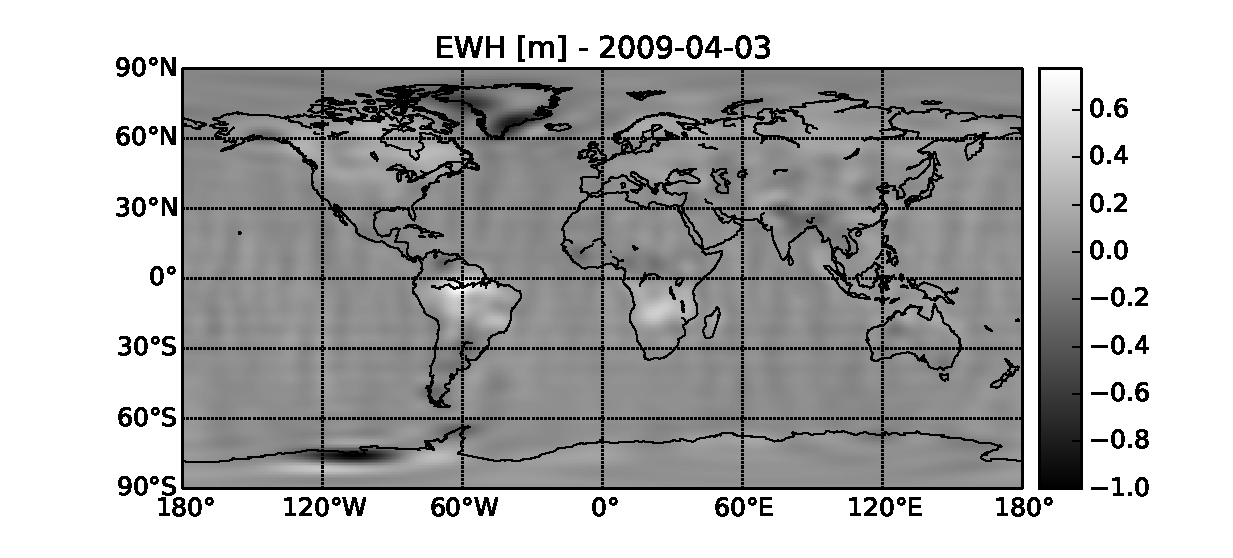
\includegraphics[width=\textwidth]{figures/data-example-world}
	\caption{Plot of the data from 3 April 2009}
	\label{fig:data-example-world}
\end{figure}

\begin{figure}[H]
	\centering
	\includegraphics[width=\textwidth]{figures/data-example-scatter}
	\caption{Plot of EWH at 63.5 N 49.5 W, west coast of Greenland.}
	\label{fig:data-example-scatter}
\end{figure}

From Figure \ref{fig:data-example-world} a local mass loss at Greenland and the South Pole is seen, this is likely caused by the ice melting.
A mass increment in South America can also been seen, this is likely caused by the rain season.
On Figure \ref{fig:data-example-scatter}, mass loss with a yearly periodic trend is seen.


\pagebreak
\section{Theory}
%!TEX root=report.tex
\subsection{SVD}
Singular Value Decomposition (SVD) is a useful method for factorizing matrixes. According to the SVD theorem a $X$ can be expressed as
\begin{equation}
X=U \Sigma V^{T}.
\label{eq:theory-svd}
\end{equation}

If the matrix $X$ have the size $m \times n$, the factorized components are \cite{introduction-to-data-mining}:
\begin{itemize}
\item The columns in $U$ are the eigenvectors of $X X^T$, with the size $m \times m$.
\item The columns in $V$ are the eigenvectors of $X^T X$, with the size $n \times n$.
\item $\Sigma$ is a diagonal matrix, consisting of the square root of the corresponding eigenvalues to the eigenvectors in $U$ and $V$.
It has the size $m \times n$. The eigenvalues are also called ``singular values''.
\end{itemize}

In the case where $X$ has have many more rows than columns, the $U$ matrix will contain more eigenvectors than what is useful and the $\Sigma$ matrix will have lots of zero-rows.
A so called \textit{economy-size} is therefore often used.
The difference being all the redundant eigenvectors in $U$ are removed, so it has the size $m \times n$ and the zero-rows from $\Sigma$ are also removed, so its size becomes $n \times n$.

An important property of SVD is that the $V$ matrix contains all eigenvectors and is therefore an orthogonal matrix, for which it known that
\begin{align}
Q^T = Q^{-1} && Q Q^T = I && Q^T Q = I && \text{, where Q is an orthogonal matrix.}
\end{align}

In the normal SVD (not \textit{economy-size}) $U$ is also a complete orthogonal matrix.
However in \textit{economy-size} some of the columns have been removed, so its only known that $U^T U = I$.

In statistics its normal to rearrange the matrices in $U \Sigma V^T$, so the largest values in $\Sigma$ appears first in the diagonal.
The reason being that $V$ is a basis matrix from the original space to another orthogonal space.
Here the first axis have the largest variance, the second axis have the second highest variance and so on.
The variance described by each axis, is given by the diagonal elements in $\Sigma^2$.
Typically this is calculated as a percentage called ``variance explained by principal components'' using
\begin{equation}
\rho_{jj} = \frac{\Sigma^2_{jj}}{\sum_{i=1}^n \Sigma^2_{ii}}.
\end{equation}

It's often seen that most of the variance can be described using very few components, thus one can reduce the dimensionality of a dataset.
These methods are called ``Principal Component Analysis (PCA)'', where a ``principal component'' should be understood as the axes in the transformed space.

%!TEX root=report.tex
\subsection{OLS}
OLS (Ordinary Least Squares) regression is used for finding the best linear transformation of one or more exogenous variables $X$ so as to predict the dependent variable $Y$. \todo{Improve formulation}
This is done by a matrix-vector product between a $\beta$ vector and $X$.
Since $X$ can be custom tailored for various purposes it is often referred to as the design matrix. The model is
\begin{align}
Y=X \beta +\epsilon && \text{, where } \mathrm{E}[\epsilon] = 0 \text{ and } \mathrm{D}[\epsilon] = \mathrm{D}[Y] = \sigma^2 I .
\end{align}

In the equation above the $\beta$-vector is the unknown parameter which needs to be determined while  $\epsilon$ is a vector containing the residuals which the model cannot account for.
Often the purpose of OLS is to predict $Y$, but in this case we want to analyze the individual $\beta_i$ elements.

\subsubsection{The solution to the OLS problem}
As the name sugest, the OLS method minimizes the sum of squared residuals ($\epsilon^T \epsilon$).
It is seen directly that $\epsilon = Y - X \beta$ and thus the following is obtained
\begin{equation}
\begin{split}
\epsilon^T\epsilon&=(Y-X\beta)^T (Y-X\beta)\\
&=(Y^T-\beta^T X^T) (Y-X\beta) \\
&=Y^T Y-\beta^T X^T Y-Y^T X \beta + \beta^T X^T X \beta \\
&=Y^T Y- 2\beta^T X^T Y+ \beta^T X^T X \beta.
\end{split}
\end{equation}

One can now differentiate with respect to the $\beta$ vector
\begin{equation}
\begin{split}
\frac{\partial \epsilon^T\epsilon}{\partial \beta}&=-2 X^T Y+2X^T X \beta=2(-X^T Y+X^T X \beta).
\end{split}
\end{equation}

Now  $\epsilon^T \epsilon$'s minimum is given by solving for $\frac{\partial \epsilon^T\epsilon}{\partial \beta} = 0$
\begin{equation}
\begin{split}
\frac{\partial \epsilon^T\epsilon}{\partial \beta} = 0 \Rightarrow 2(-X^T Y+X^T X \hat{\beta}) &= 0 \\
X^T X \hat{\beta}&=X^T Y \\
\hat{\beta}&=(X^T X)^{-1} X^T Y.
\end{split}
\end{equation}

The solution above is formally correct \cite[p.~12]{statistical-learning}, but if $X$ is badly conditioned $(X^T X)^{-1}$ might not be numerically stable (i.e., if the columns in $X$ are highly correlated leading to a near singular $X^T X$) \cite[p.~8]{aasbjerg-ls}.
To avoid this problem $X$ should be factorised and the solution reformulated; in this report we will exclusively do this using SVD
\begin{equation}
\begin{split}
\left( U \Sigma V^T\right)^T \left(U \Sigma V^T\right) \hat{\beta} &= \left(U \Sigma V^T\right)^T Y \\
V \Sigma^2 V^T \hat{\beta} &= V \Sigma U^T Y \\
\left(V \Sigma^{-2} V^T\right) V \Sigma^2 V^T \hat{\beta} &= \left(V \Sigma^{-2} V^T\right) V \Sigma U^T Y \\
\hat{\beta} &= V \Sigma^{-1} U^T Y.
\end{split}
\end{equation}

It should be noted, that when multiple $\hat{\beta}$ vectors need to be calculated (one vector for each spatial location on the surface) optimization is possible, by arranging $Y$ as a matrix with each column corresponding to a location.
$\hat{\beta}$ will then be a matrix containing all solutions instead of a vector containing only one solution.

\subsubsection{The ``Hat" matrix}
In the special case of the GRACE data, the $X$ matrix is identical for every position. This can be exploited by constructing a hat matrix $H$ which only depends on $X$ and projects $Y$ onto $\hat{Y}$ (puts the hat on $Y$).
\begin{equation}
\begin{split}
\hat{Y} &= X \hat{\beta} \Rightarrow \hat{Y} = X V \Sigma^{-1} U^T Y \\
\hat{Y} &= H Y \quad \text{, where } H = X V \Sigma^{-1} U^T.
\end{split}
\end{equation}

As earlier with $\beta$, the hat matrix can be calculated for all $Y$ vectors by vertically stacking $Y$ to form a matrix.

An important property of the $H$ matrix is that it is idempotent ($H^2 = H$) and symmetrical ($H^T = H$).
This is because $H$ is a projection matrix which projects $Y$ onto $\hat{Y}$.
Projecting $Y$ onto $\hat{Y}$ and then projecting again onto $\hat{Y}$, will obviously not change anything, because one is already in the $\hat{Y}$-plane, spanned by the columns of $X$.

\subsubsection{Root Mean Squared Error}

The ``Root Mean Squared Error'' (RMSE) is an indicator of how good an $Y$ estimate is.
It can be calculated as
\begin{equation}
\hat{\sigma} = \sqrt{\frac{\left(Y - \hat{Y}\right)^T \left(Y - \hat{Y}\right)}{n-m}},
\end{equation}

where $m$ is the number of parameters (elements in $\beta$) and $n$ is the number of observations (elements in $Y$).
RMSE is an estimate for the standard deviation of $Y$ \cite[theorem~3.4]{time-series-analysis} thus the symbol $\hat{\sigma}$.


\subsubsection{The variance of $\hat{Y}$}

The dispersion (variance-covariance) of $\hat{Y}$ can be calculated as
\begin{equation}
\mathrm{D}[\hat{Y}] = \mathrm{D}[H Y] = H \mathrm{D}[Y] H^T = \sigma^2 H^2 = \sigma^2 H.
\end{equation}

The variance of $\hat{Y_i}$ is given by the diagonal elements in $\mathrm{D}[\hat{Y}]$
\begin{equation}
\mathrm{Var}[\hat{Y_i}] = \sigma^2 H_{ii}.
\end{equation}

Because $\sigma^2$ is a scalar, the diagonal in $H$ is important to examine, since it can reveal potential elements (in our case points of time) with high variance in the predictions.

\subsubsection{The dispersion of $\hat{\boldsymbol\beta}$}

The dispersion of $\hat{\beta}$ is calculated as \cite[theorem~3.2]{time-series-analysis}:
\begin{equation}
\mathrm{D}[\hat{\beta}] = \sigma^2 (X^T X)^{-1} = \sigma^2 V \Sigma^{-2} V^T
\end{equation}

Since $\sigma^2$ is a scalar and dependent of $Y$, a similar spatial independent expression can be made, by removing the scalar $\sigma^2$  factor, thus looking exclusively at $V \Sigma^{-2} V^T$.

\subsubsection{p-values for $\hat{\boldsymbol\beta}$}

Assuming the residuals are normally distributed, the p-values for OLS parameters can be calculated using the student's t-distribution, with the t-score \cite[p.~172]{time-series-analysis}
\begin{align}
\mathrm{t} = \frac{\hat{\beta_i}}{\mathrm{SD}[\hat{\beta_i}]} && \text{where: } \mathrm{SD}[\hat{\beta_i}] = \sqrt{\mathrm{Cov}[\hat{\beta}]_{ii}} = \hat{\sigma} \sqrt{ (V \Sigma^{-2} V^T)_{ii} }.
\end{align}

Now by plugging the t-score into the Student's Cumulative distribution function ($\Phi_t$) with $N - p$ degrees of freedom, we get
\begin{equation}
p = 2 \cdot \Phi_t\left(\mathrm{abs}(t), N-p\right)
\end{equation}

The null-hypothesis is that $\beta_i = 0$ and the alternative hypothesis is $\beta_i \not = 0$.

%!TEX root=report.tex
\subsection{The design matrix}
In OLS regression, a linear combination of the columns in the design matrix,$X$,  is used to predict $Y$.
As a starting point, the only values in $X$ are a column of ones (so as to fit in intercept) and a column containing the observed time $t$:

\begin{equation}
X = \left[\begin{matrix} \mathbf{1} & \mathbf{t} \end{matrix}\right].
\end{equation}
In the above case one would end up predicting $\hat{Y}$ as  $\beta_1 + \beta_2 t$ where $\beta_1$ will correspond to the intercept (uninteresting) and $\beta_2$ will correspond to the speed of mass loss/gain.
From this it follows naturally to include the acceleration by adding a column:

\begin{equation}
X = \left[\begin{matrix} \mathbf{1} & \mathbf{t} & \frac{1}{2} \mathbf{t}^2 \end{matrix}\right]
\end{equation} 
From Fourier analysis it is know that functions can be approximated by infinite sums of the trigonometric functions; sine and cosine.
Trigonometric functions are periodic in their behaviour and thus are able to model periodic signals in the function that one wishes to approximate.

In the GRACE dataset, however, the measurements are recorded with a frequency of $\frac{1}{10}$ days.
The Nyquist-Shannon sampling theorem states that one cannot find periodic signals below the Nyquist frequency which is is given as half of the sample frequency. 
Therefore an infinite sum is not suited for approximating the function. 
Instead it will be assumed that the maximal frequency in the data has a period of a year ($365.242$ days) while the minimal frequency will have 18 periods per year since  $\sfrac{365.242}{18} \approx 20.29$. Hence it follows that the final design matrix will be given as

\begin{equation*}
\resizebox{\textwidth}{!}{$
X = \left[\begin{matrix}
	\mathbf{1} &
	\mathbf{t} &
	\frac{1}{2} \mathbf{t}^2 &
	\cos\left( \frac{2 \pi}{\frac{365.242}{1}} \mathbf{t} \right) &
	\sin\left( \frac{2 \pi}{\frac{365.242}{1}} \mathbf{t} \right) &
	\cdots &
	\cos\left( \frac{2 \pi}{\frac{365.242}{18}} \mathbf{t} \right) &
	\sin\left( \frac{2 \pi}{\frac{365.242}{18}} \mathbf{t} \right)
\end{matrix}\right].
$}
\end{equation*}


%!TEX root=report.tex
\subsection{Phase and Amplitude}

The $\hat{\beta}$ parameters in the OLS problem are coefficients in a linear combinations of $\cos(\omega_i t)$ and $\sin(\omega_i t)$ function pairs.
However, using domain knowledge from physics, having both $\cos(\omega_i t)$ and $\sin(\omega_i t)$ for the same $\omega_i$ has no meaning.
Instead one should convert the $\beta$ parameters for the trigonometric functions into amplitudes and phases corresponding to each pair of periodic functions such only a cosine  $A_i \cos(\omega_i t + \phi_i)$ is needed.
This is done by using Ptolemy's theorem
\begin{equation}
A_i \cos(\omega_i t - \phi_i) = A_i \cos(\phi_i) \cos(\omega_i t) + A_i \sin(\phi_i) \sin(\omega_i t).
\end{equation}

Comparing with the linear combination from OLS
\begin{align}
\hat{Y} = \cdots + \beta_{c,i} \cos(\omega_i t) + \beta_{s,i} \sin(\omega_i t) + \cdots
\end{align}
It is seen that
\begin{align}
\beta_{c,i} = A_i \cos(\phi_i) && \text{ and } && \beta_{s,i} = A_i \sin(\phi_i).
\end{align}

By dividing these two equations with each other, $\phi_i$ can be calculated as 
\begin{equation}
\frac{A_i \sin(\phi_i)}{A_i \cos(\phi_i)} = \frac{\beta_{s,i}}{\beta_{c,i}} \Rightarrow \phi_i = \arctan\left(\frac{\beta_{s,i}}{\beta_{c,i}}\right).
\end{equation}

To isolate $A_i$, square both equations and add them together
\begin{equation}
A_i^2 \cos(\phi_i)^2 + A_i^2 \sin(\phi_i)^2 = \beta_{c,i}^2 + \beta_{s,i}^2 \Rightarrow A_i = \sqrt{\beta_{c,i}^2 + \beta_{s,i}^2}.
\end{equation}

The result can be plotted with a circular color scale, using $\phi_i$ (the hue) and $A_i$ (the intensity).

%!TEX root=report.tex

\subsection{OLS with autocorrelated residuals}

In OLS it is assumed that the residuals between different observations are uncorrelated. However since our data is a time series this assumption does most likely not hold. This can also be confirmed with the Durbin-Watson test statistic \cite[p.~173]{autocorrelation-kousgaard}. This test statistic is calculated using
\begin{equation}
d = \frac{\sum_{i=2}^n \left( \hat{\epsilon}_i - \hat{\epsilon}_{i-1} \right)^2}{ \sum_{i=1}^n\hat{\epsilon}_i^2 }
\end{equation}

which lies between 0 and 4. If $d$ is close to 0 the residuals $\hat{\epsilon}_i$ and $\hat{\epsilon}_{i-1}$ are correlated positively, if close to 4 the residuals are negatively correlated. The purpose of this method is to reduce the correlation between the residuals, the Durbin-Watson test statistic should then become 2.

When the residuals are correlated, one gets bad estimation of the variance of the residuals $\hat{\sigma}_\epsilon^2$. This in turn leads to bad interference statistics, such as misleading p-values.

To correct for the correlated residuals, one can use a weighted least squares (WLS) regression. This uses a $\Sigma$ matrix there will correct for the correlated residuals
\begin{equation}
\min_{\beta, \rho}\ (Y-X\beta)^T \Sigma^{-1}(Y-X\beta),
\label{eq:theory-olsar-min}
\end{equation}

where $ \Sigma^{-1}$ is given as
\begin{equation}
\Sigma^{-1}  = \begin{bmatrix}
1         & -\rho         & 0               & \cdots & 0              & 0         \\
-\rho   & 1+\rho^2 & -\rho         & \cdots & 0               & 0         \\
0         & -\rho         & 1+\rho^2 & \cdots &0                & 0         \\
\vdots & \vdots      & \vdots       & \ddots & \vdots      & \vdots \\
0         & 0               &0                & \cdots & 1+\rho^2 & -\rho    \\
0         & 0               &0                & \cdots &-\rho          & 1
\end{bmatrix}
\end{equation}

The optimization problem \eqref{eq:theory-olsar-min} is nonlinear and there is no closed form solution to this problem. However when keeping $\rho$ constant the $\beta$ parameters can be estimated using Weighted Least Squared, which is similar to OLS but with a constant $\Sigma$ matrix and have the solution \cite[p.~38]{time-series-analysis}
\begin{equation}
\hat{\beta} = (X^T \Sigma^{-1} X)^{-1} X^T \Sigma^{-1} Y.
\end{equation}

This should then be rewritten using SVD, to account for a near singular $X^T \Sigma^{-1} X$ matrix.

Similarly when $\beta$ is kept constant, $\rho$ can be estimated with  \cite[p.~178]{autocorrelation-kousgaard}
\begin{equation}
\hat{\rho} = \frac{ \sum_{i=2}^n \hat{\epsilon_i}\hat{\epsilon}_{i-1} }{ \sum_{i=2}^{n-1} \hat{\epsilon_i}^2 }.
\label{eq:theory-olsar-rho}
\end{equation}

A practical way of solving the problem with respect to both $\beta$ and $\rho$, looks as follows:
\begin{enumerate}
\item initialize by letting $\rho=0$
\item Iterate: \begin{enumerate}
	\item Keep $\hat{\rho}$ constant and estimate $\beta$ using as a WLS problem.
	
	\item Keep $\hat{\beta}$ constant and estimate $\rho$ using \eqref{eq:theory-olsar-rho}.
	
	\item Repeat until convergence of $\rho$ or until some predetermined upper iteration boundary is met.
\end{enumerate}
\end{enumerate}

%!TEX root=report.tex
\subsection{Least angular regression (LAR)}
The LAR model is almost equivalent to the linear regression, except that instead of only minimizing the sum of squares, an $\ell^1$ norm penalty as added on the $\hat{\beta}$-vectors coefficients.
\begin{align}
\min_{\hat{\beta}}\ (Y - \hat{Y})^T (Y - \hat{Y}) \quad \text{subject to} \quad ||\hat{\beta}||_1 \le s
\end{align}

The LAR algorithm \cite{LAR-algorithm} solves this problem by initially letting all the $\beta$ coefficients be zero.
It then finds the attribute, $b_1$, with the highest absolute correlation with the dependent variable Y and increases $b_1$  (or decreases depending on the sign of the correlation)
until it reaches a point where another attribute $b_2$ has as much  correlation with the residuals $R=Y-\hat{Y}$ as  $b_1$ has.
At this point the algorithm then increases/decreases both $b_1$ and $b_2$ in their joint direction until another attribute $b_i$ has the highest residual correlation.
This process can then be continued until there is no benefit in increasing any of the $b_i$s - that is, the full LAR solution is equivalent to the linear regression.
It should also be noted that if a coefficient crosses 0 in a iteration (step),
that coefficient should be set to 0, and the regression direction should subsequently be recomputed.

So why might one use LAR instead of for example the LASSO model? 
When using the LASSO one has to chose a specific value of $s$ to get one solution.
However, in the LAR model you actually get the full solution path which means that you can find all the LASSO solutions instead of having to do multiple LASSO with different regularization parameters ($s$).

%!TEX root=report.tex
\subsection{Basis expansion}

Basis expansion is done by adding more columns to design matrix. Let us first motivate why this might be needed.

\subsection{Motivation}
It has previously been described how the design matrix $X$ was constructed such that we had 
\begin{equation*}
\resizebox{\textwidth}{!}{$
X = \left[\begin{matrix}
	\mathbf{1} &
	\mathbf{t} &
	\frac{1}{2} \mathbf{t}^2 &
	\cos\left( \dfrac{2 \pi}{\frac{365.242}{1}} \mathbf{t} \right) &
	\sin\left( \dfrac{2 \pi}{\frac{365.242}{1}} \mathbf{t} \right) &
	\cdots &
	\cos\left( \dfrac{2 \pi}{\frac{365.242}{18}} \mathbf{t} \right) &
	\sin\left( \dfrac{2 \pi}{\frac{365.242}{18}} \mathbf{t} \right)
\end{matrix}\right].
$}
\end{equation*}
The problem with the above $X$ is that the periodic columns assumes the pattern accounts for the entire period. This causes problems in areas such as Denmark, where the winter comes later than ``usual'', or the summer is much colder/warmer etc..

This leads to higher variance of the residuals which decreases the accuracy of the velocity and acceleration parameter of the model. By adding columns to the design matrix, such that the periodic pattern is only assumed extend over one period, the accuracy can be improved.

\subsection{The Hinge-function}

One can achieve this basis expansion is by virtue of the hinge-function
\begin{equation}
f(x - \zeta)_+ = \begin{cases}
  f(x - \zeta) & \text{if } x - \zeta \ge 0 \\
  0                 & \text{otherwise}
\end{cases} \quad \forall x \in \mathbb{R}, \zeta \in \mathbb{R}
\end{equation}
$\zeta$ denotes the ``knot'' between the zero part and the $f$ part. By choosing $f$ and adding the hinge function to the design matrix, a basis expansion where terms are only active for some parts of the time series is obtained.

When $f$ is a polynomial one achieve a piecewise polynomial which is called a spline.
In this case each hinge function is guaranteed to be continuous and it can be shown that the spline's derivatives are continuous to order $M-2$ where $M$ is the degree of polynomial $f$ \cite[p.~144]{statistical-learning}. When dealing with polynomials, splines which are continuous up to and including its second order derivatives are called \textit{cubic splines} and they generate nicely looking curves when performing the regression. \cite[p.~143]{statistical-learning}.

\subsubsection{Knots and trigonometric functions}
To model each year with different behavior, in essence all that is needed is to create 9 knots (10 intervals requires 9 splits) and construct the hinge functions.
However, since the functions being used are sines and cosines, there is no guarantee of continuity at the knots (only continuity if the trigonometric function evaluates to zero at the knot).
In grim cases, when multiple discontinuous functions are combined, one can end up with cusps, that is a steep descent/ascend followed by the opposite movement in rapid succession.
If this phenomenon becomes too large, one should consider rejecting the model, this will be discussed in the result section. 

%!TEX root=report.tex
\subsection{Time Series Analysis}

In time series analysis one attempt to find a model for predicting data. This is different form the OLS analysis there tries to estimate the trends in the data, such as velocity and acceleration. Once such model is found, it should be validated by analyzing the residuals. These residuals must be approximately white noise \cite[p.~130]{time-series-analysis}, otherwise the model is invalid. 

\subsubsection{ARIMA}

ARIMA is the name of the stochastic model used. The detail will not be discussed here, instead we refer to \cite[p.~130]{time-series-analysis}.

In short ARIMA uses the previous values with some weight to predict. Which values are used is denoted by the following notation:
\begin{equation}
(p, d, q) \times (P, D, Q)_s
\end{equation}

$p$ is the highest lags of actual measurements used and $q$ is the maximum amount of lags in residuals used. The $d$ part indicates how many difference operators there should be used to transform the data. $(P, D, Q)$ is completely similar, but steps not by one lag but by $s$ lags. This allows for seasons trends such as an yearly pattern.

\subsubsection{ACF and PACF}
 
ACF and PACF is a measure of correlation between different time lags and is used to make a qualified guess about how the predicting model should look like. 
For how these are estimation please see \cite[p.~146]{time-series-analysis}.

When ACF and PACF have been estimated, rules \cite[table~6.1]{time-series-analysis} for how the stochastic model should look can be applied.
Typically when dealing with complex models, this becomes and iterative process.
Where one will calculate the ACF and PACF on the suggested model and then adjust the model accordingly.

\subsection{Ljung-Box test}

The null hypothesis for the Ljung-Box is ``The data is independently distributed''. Thus a low p-value means that the residuals aren't white noise.

The Ljung-Box is a $\chi^2$ test with the statistical value:
\begin{equation}
Q = n \cdot (n + 2) \sum_{k=1}^h \frac{\hat{\rho}_k^2}{n - k}
\end{equation}

$n$ is the number of observations. The parameter $h$ is the highest lag in the ACF there should be considered. The $\chi^2$ statistics, have $h - (p + q + P + Q)$ degrees of freedom.

%!TEX root=report.tex
\subsection{K-means clustering}

Clustering is the process of grouping or dividing a set of objects into disjunct subsets, such that objects in each cluster are similar.
All clustering methods are unsupervised learning methods, thus there is no ``correct'' answer.
It have been shown that given a set of objects, humans also differ in their choice of clusters.

Since similarity is an imprecise term, one uses a distance function to use as a Dissimilarity Measure $d$.

There are 4 conditions a distance function $d$ must satisfy, they are all derived from the norm definition \cite[p.~30]{math-4}:
\begin{align}
\text{(i) }   & d(p_1,p_2) \ge 0 && \forall \ p_1, p_2 \in V \\
\text{(ii) }  & d(p_1,p_2) \le d(p_1, p_3) + d(p_3, p_2) && \forall \ p_1, p_2, p_3 \in V \\
\text{(iii) } & d(p_1, p_2) = d(p_2, p_1) && \forall \ p_1, p_2 \in V \\
\text{(iv) } & d(p_1, p_2) = 0 \Leftrightarrow p_1 = p_2 && \forall \ p_1, p_2 \in V
\end{align}

Given a distance measure the total cluster variance $C^{*}$ can be calculated as
\begin{equation}
C^{*}=\sum^K_{k=1} N_k \sum_{i \in C_k} D(x_i-\mu_k).
\end{equation}
Here $\mu_k$ denotes the k\textsuperscript{th} cluster center (also called a centroid), $N_k$ the number of observations in cluster $k$ and $C_k$ denotes the subset with all the points in the cluster $k$.

In this analysis the Euclidean distance $d(p_i, p_j)= \sqrt{(p_i-p_j)(p_i-p_j)^{T}}$ has been chosen as the dissimilarity measure.
K-means is then the chosen algorithm for minimizing $C^{*}$ given $K$ clusters.
The k-means method as the dataset size is $(lat \cdot lon, days) = (64800,341)$ and k-means is fairly quick to converge and calculate.

K-means makes a single big assumption about the clusters being hyper dimensional sphere. But beyond this K-means is a simple iterative algorithm:
\begin{enumerate}
	\item Initialize cluster centroids
	\item Iterate until centroid convergence:
	\begin{enumerate}
		\item Given the current set of centroids, reassign each observation to the closest centroid using the distance function.
		\item Using the current cluster assignment $C_k\ \forall k$, minimize $C^{*}$ by recomputing the centroids for each cluster as the mean of points in each cluster.
	\end{enumerate}
\end{enumerate}

\subsubsection{Gap-statistics}

The big issue with clustering is that there is no obvious way of selecting the amount of clusters $K$. In this analysis the Gap-statistics \cite[p.~519]{statistical-learning} as proposes by Hastie, Tibshirani and Firedman is used.

First calculate the cluster dissimilarity using $K$ clusters \cite{gap-statistic}
\begin{equation}
W_K = \sum_{k=1}^K \frac{1}{2 N_k} \sum_{x_i\in C_k} \sum_{x_j\in C_k} d(x_i,x_j).
\end{equation}

Given the quantity $W_k$ one can then calculate a gap $G$ by simulating $b$ datasets from a random uniform distribution and calculating the gap as
\begin{equation}
G(k) = \mathrm{E}[\log(W_k)] - \log(W_k),
\end{equation}
where the expectation $E[log W_k]$ can be estimated by the mean over the $b$ simulated datasets. That is the gap statistics tries to avoid overfitting by comparing the cluster gain on a dataset where there are no clusters (uniformly distributed).

The amount of clusters $K$ is then minimized under the condition
\begin{equation}
K^{*} = \argmin_K \left\{ K \ | \ G(K) \ge G(K + 1) - s'_{K} \right\}.
\end{equation}

Here $s'_{K+1}$ is the standard error on the $b$ samples calculated as 
\begin{equation}
s'_{K} = \mathrm{SD}[\log(W_k)] \sqrt{1+\frac{1}{b}}.
\end{equation}

%!TEX root=report.tex
\subsection{The Gaussian Mixture Model (GMM)}

The GMM is a more advanced clustering model than KMeans. 
The main advantage is that there are no restrictions on each cluster's covariance matrix where as the reader remembers that KMeans clusters had a diagonal covariance structure. 
Such restrictions (i.e. shared covariance, diagonal covariance, spherical covariance etc.) can relatively easily be applied in the GMM if one so chooses; here, however, only the case with no covariance restrictions will be described.
\\
In the GMM each cluster is viewed as a Gaussian density function. 
This density has a centroid (Just as with KMeans) and a covariance matrix.
The density function is assumed to be a combination (mixture) of $K$ Gaussian PDFs (Probability Density Function) where K is finite.


In practice if K is large and the vector space has is high dimensional 

\subsubsection{Dimensionality reduction}
%!TEX root=report.tex
\subsection{Kernel PCA}

Before delving into kernel methods, the standard PCA method will briefly be recapped.
PCA as introduced in this report was done via SVD ($X = U\Sigma V^T$). The columns of $U$ is the eigenvectors of $XX^T$. The projected space is then $Z = XV = U\Sigma$. 
Looking at the dependencies of $U$, it is apparent that the principal component scores, will end up being linear combinations of basis in original input space $X$. 
In most cases this suffices but what if there are no linear relationships in the $X$ space, standard PCA won't be appropriate.

\subsubsection{Motivating example}
\begin{figure}[H]
	\center
	\includegraphics[width=\textwidth]{figures/kernel-pca-example}
	\caption{Motivating kernel PCA example. Image courtesy of scikit-learn. License: BSD 3 clause. Authors: Mathieu Blondel and Andreas Mueller.}
	\label{fig:kernel-pca-example}
\end{figure}

As is seen in Figure \ref{fig:kernel-pca-example}, classes that wasn't linearly separable in the original space can be become linearly separable in the kernel space. This in turn makes clustering much easier and hopefully improves results.

\subsubsection{The Kernel Trick}

In kernel PCA, instead of working on $X X^T$, a nonlinear mapping $\Phi: X\rightarrow Y$ is used, such that the SVD is carried out on $\Phi(X)\Phi(X)^T = K(X, X^T)$. Specifically one define the inner product as a function of $(x_i, x_j)$, thus $\Phi(X)\Phi(X)^T$ is calculated, but without the need for the nonlinear mapping function $\Phi$. This inner product function is the kernel.
 
For something to be a valid kernel, all the kernel needs to satisfy is to be function of an inner product in some vector space.
For the above to become more clear, let us give an example of a polynomial kernel in a 2-dimensional space. in the following $X$ is a vector and $X'$ is simply some other vector in the same space as $X$:
\begin{equation}
\begin{split}
K(X,X') &= (1+X^T X')^2 = (1+x_1 x'_1+x_2 x'_2)^2 \\
&= 1+x_1^2 {x'}_1^2 +2 x_1 x'_1 + 2 x_2 x'_2 + 2 x_1 x'_1 x_2 x'_2
\end{split}
\end{equation}

For the above to actually be a actual kernel there would have to be some transformed space in which the above was an inner product. From the coefficients above it can be deduced that the basis in this transformed space must be given as
\begin{equation}
(1,x_1^2,x_2^2,\sqrt{2} x_1, \sqrt{2} x_2 , \sqrt{2} x_1 x_2)
\end{equation}

Now consider if one used a power of 100 instead of 2. Calculating the kernel in the non transformed  space is easy; $(1+X^T X')$ is just a number and raising it to the power of 100 can be done quickly.
On the other hand if one were to explicitly calculate the kernel as the inner product in the transformed space, a huge vector would have to be computed, transposed and be subjected to an the inner product in this space. This is clearly not very efficient.

The shortcut to define $K$ instead of $\Phi$ is called the Kernel Trick.

\subsubsection{The Radial Basis Function (RBF) kernel}

The RBF kernel is commonly used when the amount of samples is much larger than the amount of dimensions in the original space.

The RBF kernel is defined as
\begin{equation}
K(x,x')=\mathrm{exp}(-\gamma ||x-x'||^p_2)
\end{equation}

The above can easily be calculated. The following shows that the above is indeed an inner product. It is not a complete proof as $\gamma=1, p=2$ and $x$ is a scalar not a vector.

\begin{equation}
\begin{split}
	K(x,x')&=\mathrm{exp}(- ||x-x'||^2_2)=\mathrm{exp}(- (x-x')^2) \\
		  &= \mathrm{exp}(-x^2) \mathrm{exp}(-{x'}^2) \mathrm{exp}(2 x x')
\end{split}
\end{equation}
since $\mathrm{exp}(2 x x')$ can be Taylor expanded to $\sum_{k=0}^\infty \frac{2^k(x)^k (x')^k}{k!}$ it follows that:
\begin{equation}
K(x,x') = \sum_{k=0}^\infty \left(\sqrt{\frac{2^k}{k!}} (x)^k \mathrm{exp}(-x^2)\right)\left(\sqrt{\frac{2^k}{k!}} (x')^k \mathrm{exp}(-{x'}^2)\right)
\end{equation}

From the above it is seen that for any k, the term in the right parenthesis is exactly equal to the left parenthesis, if $x'$ was substituted with $x$. This means that in an expanded vector space, this correspond to the the inner product from the $\ell^2$ Hilbert space. Do also note that since the sum is infinite, the transformed vector space is of infinite dimensional space and is thus impossible to calculate without the kernel trick.

\subsubsection{Mercer's Condition}
Proving that something is a kernel, is actually easier than shown above. It is done using Mercer's Condition, though it does not say anything about the size of the transformed space when $\Phi$ is applied.

The theorem states, that given all real valued square integrable functions $g$ (${g \in \{\mathbb{R} \rightarrow \mathbb{R}\} \cap L^2(\mathbb{R})}$). That is the following must be true:
\begin{equation}
\int_{-\infty}^{\infty} g(x)^2 \mathrm{d}x < \infty
\end{equation}

Then for all these $g$ functions, if the following condition holds:
\begin{equation}
\int \int K(x, y) g(x) g(y) \mathrm{d}x \mathrm{d}y \ge 0
\end{equation}

Then $K$ is a valid kernel.

\subsubsection{Final notes of kernel PCA}

In kernel PCA the columns of $U$ is the eigenvectors of $K(X,X^T)$ and the columns of $V$ the eigenvectors of $K(X^T,X)$. The size of $X X^T$ and $X^T X$ is going to be $nxn$ and $pxp$ respectively where $n$ is the number of samples and $p$ the dimensions in transformed space. Thus when dealing with kernel PCA the calculation of $V$ is omitted and calculation of $U$ is expensive, but possible.

In the case of the GRACE data the size of $X$ is ($64800 \times 341$). Memory wise this results in a $U$ matrix of size ($64800 \times 64800$) with float32 numbers, that is approximately $15.64\text{ GB}$. Furthermore kernel PCA also involves quite a lot of simple computing. So for practical purposes one should use a computer cluster (e.q. the DTU HPC cluster).


\pagebreak
\section{Results}
%!TEX root=report.tex
\subsection{OLS}

The first part of the OLS analysis will examine the EWH at two specific locations. The second part will then focus on the entire world. The main purpose of the OLS analysis is to estimate the velocity and acceleration of the mass changes. 

\subsubsection{Selected locations}

The two selected locations are:
\begin{itemize}
\item Greenland ($63.5^\circ$ N, $49.5^\circ$ W)
\item Western Antartica ($74.5^\circ$ S, $87.5^\circ$ W)
\end{itemize}
\begin{figure}[H]
	\centering
	\includegraphics[height=6cm]{figures/ols-selected-map}
	\caption{The two selected locations, marked with a red star}
\end{figure}

\paragraph{Greenland}

At the west coast of Greenland a strong period trend can be observed, probably caused by the the ice melting over the summer and reappearing during the winter. This trend is seen in Figure \ref{fig:ols-selected-0-fit}. In order to estimate the velocity and acceleration of the EWH accurately, it is important that the periodic trend is caught by the $\sin(\cdot)$ and $\cos(\cdot)$ terms so that seasonal patterns do not interfere with the estimates.
\begin{figure}[H]
	\centering
	\includegraphics[width=\textwidth]{figures/ols-selected-0-fit}
	\caption{Measurements are blue, the OLS fit is red.}
	\label{fig:ols-selected-0-fit}
\end{figure}
 
From Figure \ref{fig:ols-selected-0-fit} it's seen that the period trend is caught by the model, however for some seasons (particularly between 2008 and 2010) the fit is not very good. This is even more clear when looking at the residuals in Figure \ref{fig:ols-selected-0-residual}. From this it is clear that the residuals are far from white noise, which was one of the OLS assumptions.
\begin{figure}[H]
	\centering
	\includegraphics[width=\textwidth]{figures/ols-selected-0-residual}
	\caption{The OLS residuals are blue.}
	\label{fig:ols-selected-0-residual}
\end{figure}

In addition to the yearly season, when looking at the estimated OLS coefficients (Table \ref{table:ols-selected-0-paramters}) there also seems to be a half yearly season. Though strangely enough it is not very visible on the OLS fit (Figure \ref{fig:ols-selected-0-fit}). The remaining seasons are with 95\% confidence not significantly different from zero and for the purpose of getting a better estimate, it might be worth iteratively removing these parameters.
\begin{table}[H]
\centering
\centerline{\begin{tabular}{r|rr}
\hline
 name                           & estimate               & p-value   \\
\hline
 $intercept (1)$                & $-1.77 \cdot 10^{-01}$ & $0.000$   \\
 $vel. (t)$                     & $-2.24 \cdot 10^{-04}$ & $0.000$   \\
 $acc. (0.5 \cdot t^2)$         & $-8.27 \cdot 10^{-08}$ & $0.000$   \\
 $\cos(1 \cdot \omega \cdot t)$ & $-1.35 \cdot 10^{-02}$ & $0.000$   \\
 $\sin(1 \cdot \omega \cdot t)$ & $-8.28 \cdot 10^{-02}$ & $0.000$   \\
 $\cos(2 \cdot \omega \cdot t)$ & $-5.86 \cdot 10^{-03}$ & $0.045$   \\
 $\sin(2 \cdot \omega \cdot t)$ & $-1.41 \cdot 10^{-02}$ & $0.000$   \\
 $\cos(3 \cdot \omega \cdot t)$ & $-5.01 \cdot 10^{-03}$ & $0.089$   \\
 $\sin(3 \cdot \omega \cdot t)$ & $-5.69 \cdot 10^{-03}$ & $0.053$   \\
 $\cos(4 \cdot \omega \cdot t)$ & $-5.49 \cdot 10^{-03}$ & $0.060$   \\
 $\sin(4 \cdot \omega \cdot t)$ & $-1.66 \cdot 10^{-03}$ & $0.573$   \\
 $\cos(5 \cdot \omega \cdot t)$ & $-2.19 \cdot 10^{-03}$ & $0.455$   \\
 $\sin(5 \cdot \omega \cdot t)$ & $-1.93 \cdot 10^{-03}$ & $0.511$   \\
 $\cos(6 \cdot \omega \cdot t)$ & $4.29 \cdot 10^{-04}$  & $0.883$   \\
 $\sin(6 \cdot \omega \cdot t)$ & $1.43 \cdot 10^{-03}$  & $0.627$   \\
 $\cos(7 \cdot \omega \cdot t)$ & $9.55 \cdot 10^{-04}$  & $0.744$   \\
 $\sin(7 \cdot \omega \cdot t)$ & $1.09 \cdot 10^{-04}$  & $0.970$   \\
 $\cos(8 \cdot \omega \cdot t)$ & $-3.08 \cdot 10^{-04}$ & $0.916$   \\
 $\sin(8 \cdot \omega \cdot t)$ & $-2.37 \cdot 10^{-04}$ & $0.935$   \\
 $\cos(9 \cdot \omega \cdot t)$ & $-2.02 \cdot 10^{-03}$ & $0.491$   \\
\hline
\end{tabular}\hspace{1cm}\begin{tabular}{r|rr}
\hline
 name                            & estimate               & p-value   \\
\hline
 $\sin(9 \cdot \omega \cdot t)$  & $8.48 \cdot 10^{-04}$  & $0.772$   \\
 $\cos(10 \cdot \omega \cdot t)$ & $1.54 \cdot 10^{-03}$  & $0.599$   \\
 $\sin(10 \cdot \omega \cdot t)$ & $-5.77 \cdot 10^{-04}$ & $0.843$   \\
 $\cos(11 \cdot \omega \cdot t)$ & $-5.95 \cdot 10^{-04}$ & $0.839$   \\
 $\sin(11 \cdot \omega \cdot t)$ & $-1.47 \cdot 10^{-03}$ & $0.615$   \\
 $\cos(12 \cdot \omega \cdot t)$ & $1.78 \cdot 10^{-04}$  & $0.952$   \\
 $\sin(12 \cdot \omega \cdot t)$ & $5.37 \cdot 10^{-04}$  & $0.854$   \\
 $\cos(13 \cdot \omega \cdot t)$ & $2.57 \cdot 10^{-03}$  & $0.383$   \\
 $\sin(13 \cdot \omega \cdot t)$ & $-6.35 \cdot 10^{-04}$ & $0.827$   \\
 $\cos(14 \cdot \omega \cdot t)$ & $3.16 \cdot 10^{-04}$  & $0.914$   \\
 $\sin(14 \cdot \omega \cdot t)$ & $-2.99 \cdot 10^{-04}$ & $0.919$   \\
 $\cos(15 \cdot \omega \cdot t)$ & $-7.23 \cdot 10^{-04}$ & $0.804$   \\
 $\sin(15 \cdot \omega \cdot t)$ & $3.33 \cdot 10^{-04}$  & $0.910$   \\
 $\cos(16 \cdot \omega \cdot t)$ & $-8.07 \cdot 10^{-04}$ & $0.785$   \\
 $\sin(16 \cdot \omega \cdot t)$ & $-6.93 \cdot 10^{-04}$ & $0.811$   \\
 $\cos(17 \cdot \omega \cdot t)$ & $-1.26 \cdot 10^{-03}$ & $0.665$   \\
 $\sin(17 \cdot \omega \cdot t)$ & $-7.28 \cdot 10^{-04}$ & $0.803$   \\
 $\cos(18 \cdot \omega \cdot t)$ & $-4.93 \cdot 10^{-04}$ & $0.864$   \\
 $\sin(18 \cdot \omega \cdot t)$ & $-9.94 \cdot 10^{-06}$ & $0.997$   \\
                                 &                        &           \\
\hline
\end{tabular}}
\caption{Parameter estimates $\hat{\beta}$ and their p-values for Greenland.}
\label{table:ols-selected-0-paramters}
\end{table}

\paragraph{Western Antarctica}

Just like with Greenland there is a clear drop in mass as seen in Figure \ref{fig:ols-selected-1-fit}. Interestingly enough, there is no seasonal trend or at least it is not very strong. Also the existence of high frequency terms in the OLS regression, is more apparent. Though from the actual data it does not look like such periodic trends exist. This suggests that too many seasonal parameters have been used, thus causing some overfitting.
\begin{figure}[H]
	\centering
	\includegraphics[width=\textwidth]{figures/ols-selected-1-fit}
	\caption{Measurements are blue, the OLS fit is red.}
	\label{fig:ols-selected-1-fit}
\end{figure}

When looking at the residuals in Figure \ref{fig:ols-selected-1-residual}, it is again clear that the residuals are far from being white noise. There also seems to be some periodic trend in the residuals; that is the residuals appear to have a seasonal pattern. However, the beginnings and the endings of these seasons are quite hard to make out. 

\begin{figure}[H]
	\centering
	\includegraphics[width=\textwidth]{figures/ols-selected-1-residual}
	\caption{The OLS residuals are blue.}
	\label{fig:ols-selected-1-residual}
\end{figure}

Just as with Greenland many of the OLS terms are with 95\% confidence not significantly different from zero. Interestingly enough there is a yearly season when looking at Table \ref{table:ols-selected-1-paramters}, though it's very hard to make out from the OLS fit in Figure \ref{fig:ols-selected-1-fit}.

\begin{table}[H]
\centering
\centerline{\begin{tabular}{r|rr}
\hline
 name                           & estimate               & p-value   \\
\hline
 $intercept (1)$                & $-1.38 \cdot 10^{-01}$ & $0.000$   \\
 $vel. (t)$                     & $-2.26 \cdot 10^{-04}$ & $0.000$   \\
 $acc. (0.5 \cdot t^2)$         & $-1.24 \cdot 10^{-07}$ & $0.000$   \\
 $\cos(1 \cdot \omega \cdot t)$ & $1.69 \cdot 10^{-02}$  & $0.000$   \\
 $\sin(1 \cdot \omega \cdot t)$ & $1.42 \cdot 10^{-02}$  & $0.000$   \\
 $\cos(2 \cdot \omega \cdot t)$ & $-7.19 \cdot 10^{-03}$ & $0.046$   \\
 $\sin(2 \cdot \omega \cdot t)$ & $2.82 \cdot 10^{-03}$  & $0.440$   \\
 $\cos(3 \cdot \omega \cdot t)$ & $-4.36 \cdot 10^{-03}$ & $0.227$   \\
 $\sin(3 \cdot \omega \cdot t)$ & $-1.23 \cdot 10^{-03}$ & $0.732$   \\
 $\cos(4 \cdot \omega \cdot t)$ & $1.78 \cdot 10^{-03}$  & $0.619$   \\
 $\sin(4 \cdot \omega \cdot t)$ & $2.81 \cdot 10^{-03}$  & $0.437$   \\
 $\cos(5 \cdot \omega \cdot t)$ & $2.45 \cdot 10^{-03}$  & $0.496$   \\
 $\sin(5 \cdot \omega \cdot t)$ & $2.53 \cdot 10^{-03}$  & $0.484$   \\
 $\cos(6 \cdot \omega \cdot t)$ & $-1.60 \cdot 10^{-03}$ & $0.654$   \\
 $\sin(6 \cdot \omega \cdot t)$ & $-8.66 \cdot 10^{-04}$ & $0.811$   \\
 $\cos(7 \cdot \omega \cdot t)$ & $8.95 \cdot 10^{-04}$  & $0.803$   \\
 $\sin(7 \cdot \omega \cdot t)$ & $-3.27 \cdot 10^{-03}$ & $0.364$   \\
 $\cos(8 \cdot \omega \cdot t)$ & $1.62 \cdot 10^{-03}$  & $0.652$   \\
 $\sin(8 \cdot \omega \cdot t)$ & $-1.51 \cdot 10^{-03}$ & $0.674$   \\
 $\cos(9 \cdot \omega \cdot t)$ & $3.76 \cdot 10^{-04}$  & $0.917$   \\
\hline
\end{tabular}\hspace{1cm}\begin{tabular}{r|rr}
\hline
 name                            & estimate               & p-value   \\
\hline
 $\sin(9 \cdot \omega \cdot t)$  & $2.05 \cdot 10^{-03}$  & $0.568$   \\
 $\cos(10 \cdot \omega \cdot t)$ & $-4.54 \cdot 10^{-04}$ & $0.900$   \\
 $\sin(10 \cdot \omega \cdot t)$ & $-1.26 \cdot 10^{-03}$ & $0.726$   \\
 $\cos(11 \cdot \omega \cdot t)$ & $-1.21 \cdot 10^{-04}$ & $0.973$   \\
 $\sin(11 \cdot \omega \cdot t)$ & $-1.07 \cdot 10^{-03}$ & $0.766$   \\
 $\cos(12 \cdot \omega \cdot t)$ & $-1.20 \cdot 10^{-03}$ & $0.740$   \\
 $\sin(12 \cdot \omega \cdot t)$ & $-8.20 \cdot 10^{-04}$ & $0.819$   \\
 $\cos(13 \cdot \omega \cdot t)$ & $-5.73 \cdot 10^{-03}$ & $0.114$   \\
 $\sin(13 \cdot \omega \cdot t)$ & $-8.50 \cdot 10^{-04}$ & $0.812$   \\
 $\cos(14 \cdot \omega \cdot t)$ & $-6.55 \cdot 10^{-04}$ & $0.855$   \\
 $\sin(14 \cdot \omega \cdot t)$ & $2.25 \cdot 10^{-03}$  & $0.533$   \\
 $\cos(15 \cdot \omega \cdot t)$ & $-4.32 \cdot 10^{-04}$ & $0.904$   \\
 $\sin(15 \cdot \omega \cdot t)$ & $3.05 \cdot 10^{-04}$  & $0.933$   \\
 $\cos(16 \cdot \omega \cdot t)$ & $3.51 \cdot 10^{-04}$  & $0.923$   \\
 $\sin(16 \cdot \omega \cdot t)$ & $-3.73 \cdot 10^{-04}$ & $0.917$   \\
 $\cos(17 \cdot \omega \cdot t)$ & $1.22 \cdot 10^{-03}$  & $0.735$   \\
 $\sin(17 \cdot \omega \cdot t)$ & $-1.11 \cdot 10^{-03}$ & $0.758$   \\
 $\cos(18 \cdot \omega \cdot t)$ & $-1.92 \cdot 10^{-04}$ & $0.957$   \\
 $\sin(18 \cdot \omega \cdot t)$ & $7.18 \cdot 10^{-04}$  & $0.844$   \\
                                 &                        &           \\
\hline
\end{tabular}}
\caption{Parameter esimates $\hat{\beta}$ and their p-values for Greenland. }
\label{table:ols-selected-1-paramters}
\end{table}

\pagebreak
\subsubsection{World view}

\paragraph{Parameters}

As mentioned earlier, the velocity and acceleration of the mass changes are the most important parameters in the OLS regression.
\begin{figure}[H]
	\centering
	\includegraphics[width=\textwidth]{figures/ols-world-parameter-vel}
	\caption{Estimated velocity ($t$) parameters}
	\label{fig:ols-world-parameter-vel}
\end{figure}

\begin{figure}[H]
	\centering
	\includegraphics[width=\textwidth]{figures/ols-world-parameter-acc}
	\caption{Estimated acceleration ($\frac{1}{2} t^2$) parameters}
	\label{fig:ols-world-parameter-acc}
\end{figure}

The first two figures (Figure \ref{fig:ols-world-parameter-vel} and Figure \ref{fig:ols-world-parameter-acc}) show that, generally there is a mass loss at both Greenland and the Western Antarctica and that it is accelerating. However interestingly enough the East Coast of Greenland do not show any acceleration, maybe even a slight deceleration of the mass loss (a positive value).

On both figures there is also a circular pattern at Thailand (10 N, 95 E), which is caused by the infamous earthquake of the 26th December 2004, resulting in significant changes in the mass distribution, thus affecting the data from GRACE.
\begin{figure}[H]
	\centering
	\includegraphics[width=\textwidth]{figures/ols-world-parameter-year}
	\caption{Intensity-Hue plot. Estimated phase controls the hue while the amplitude sets the intensity.}
	\label{fig:ols-world-parameter-year}
\end{figure}

The seasonal trends do not reveal any information about mass loss due to ice melting, since this is something which will continue to have effect for many years. However it does affect the estimation of the velocity and acceleration. Also having more season related terms in the OLS regression than necessary, will result in fewer degrees of freedom.

In Figure \ref{fig:ols-world-parameter-year} it is seen from the intensity, that the Western Antarctica do not have a strong yearly seasonal trend unlike Greenland. It also appears that it is primarily the East Coast of Greenland which has a yearly seasonal trend. The strongest seasonal trend appears in South America (more specifically the Amazon Basin), and this is due to the rain season. This rain also takes quite some time to reach the ocean, thus causing the phase gradient.

\paragraph{Performance} 

As a measure of  model performance the root mean squared error has been calculated for each position.
\begin{figure}[H]
	\centering
	\includegraphics[width=\textwidth]{figures/ols-world-performance-rmse}
	\caption{RMSE for each position.}
	\label{fig:ols-world-performance-rmse}
\end{figure}

From \ref{fig:ols-world-performance-rmse} it is seen that the hardest places to fit are South America and Thailand. In South America it is especially around the Amazon River that the RMSE is high. This suggests that it is caused by changes in the rain seasons, since this is also the place with the highest amplitude of the yearly seasonal term. It's a bit odd that this is so hard to fit, since the model does support seasonal trends. One explanation could be that this OLS model assumes that the season are equally long and with identical phases each year, which is not very likely. The circular pattern around Thailand is no surprise, since the OLS model was never meant to fit this distortion.

Neither of these issues are related to the ice melting, which makes them less important. However the East Coast of Greenland and the Western Antarctica also show a relative higher RMSE, when comparing to the ocean or the nearby land, which is less than ideal. The fact that it is primarily the East Coast of Greenland and not the west coast, suggests that the issues are related to the seasons, just like with the Amazon Basin. This was also something observed, when looking at the specific location's time series.

\paragraph{Standard diagnostics} Recalling that $\mathrm{Var}[\hat{Y}_i] = \sigma^{2} H_{ii}$ and $\mathrm{D}[\hat{\beta}] = \sigma^{2} V \Sigma^{-2} V^T$ the diagonal of $H$ and $V \Sigma^{-2} V^T$ are both important to examine. This will identify any days and parameters with high variance (the reader should remember that is applies to all positions).

\begin{figure}[H]
	\centering
	\includegraphics[width=\textwidth]{figures/ols-world-diagnostics-diagH}
	\caption{The diagonal of $H$ will reveal any days with a high variance.}
	\label{fig:ols-world-performance-diagH}
\end{figure}

The variances shown in Figure \ref{fig:ols-world-performance-diagH} are not very big, the highest is $0.16$ and recalling that the 95\% confidence interval can be approximated by $\hat{Y}_i \pm 2 \cdot \hat{\sigma} \sqrt{\mathrm{Var}[\hat{Y}_i]}$. The maximal confidence interval becomes $\hat{Y}_i \pm 2 \cdot 0.135 \cdot \sqrt{0.16} = \hat{Y}_i \pm 0.108$, which is small when comparing to the EWH values, which range from $1$ to $-3$. What is odd about $\mathrm{diag}(H)$ is that there appears to be some parts in each year which are more difficult to predict than others. \todo{Why is this}

\begin{figure}[H]
	\centering
	\includegraphics[height=9cm]{figures/ols-world-diagnostics-cov}
	\caption{Colleration matrix reveals correlated parameter.}
	\label{fig:ols-world-performance-cov}
\end{figure}

From Figure \ref{fig:ols-world-performance-cov} it is seen that the parameters are nicely uncorrelated and while the seasonal parameters have a slightly high variance when comparing to their values; the variation of the velocity and the acceleration parameters are practically zero.
\begin{table}[H]
\centering
\begin{tabular}{r|c c c}
	name & $\mathrm{Var}[\hat{\beta}_i]$ \\ \hline
	$vel. (t)$ & $2.91390457 \cdot 10^{-09} [\frac{m^2}{day^2}]$  \\
	$acc. (0.5 \cdot t^2)$ & $1.29525397 \cdot 19^{-14} [\frac{m^2}{day^4}]$
\end{tabular}
\caption{Variance of the velocity and acceleration parameters for all positions .}
\end{table}
\todo{Check that this is really true}
\paragraph{p-values} Just as for the selected positions, inspecting the p-values can tell which OLS terms are important.

\begin{figure}[H]
	\centering
	\includegraphics[width=\textwidth]{figures/ols-world-diagnostics-pvalue-1}
	\caption{p-values for the velocity parameter.}
	\label{fig:ols-world-diagnostics-pvalue-1}
\end{figure}

\begin{figure}[H]
	\centering
	\includegraphics[width=\textwidth]{figures/ols-world-diagnostics-pvalue-2}
	\caption{p-values for the acceleration parameter.}
	\label{fig:ols-world-diagnostics-pvalue-2}
\end{figure}

There is not much surprise in either Figure \ref{fig:ols-world-diagnostics-pvalue-1} or Figure \ref{fig:ols-world-diagnostics-pvalue-2}. Both the velocity and the acceleration appears to be significant pretty much everywhere. The places where it is not, is where there is a sign shift thus causing the p-value gradient. This is particularly apparent with the acceleration. One odd detail is that also on the ocean, the velocity and acceleration parameters appears to be significantly different from zero. In the ocean there is no reason to expect a steady mass change, though when looking at actual values it's seen that there is a slight slope. This quite small slope then becomes significant, due to the very small variance of the velocity and acceleration parameters. 

\begin{figure}[H]
	\centering
	\includegraphics[width=\textwidth]{figures/ols-world-diagnostics-pvalue-3}
	\caption{p-values for the yearly seasonal cosine parameter.}
	\label{fig:ols-world-diagnostics-pvalue-3}
\end{figure}

\begin{figure}[H]
	\centering
	\includegraphics[width=\textwidth]{figures/ols-world-diagnostics-pvalue-4}
	\caption{p-values for the yearly seasonal sine parameter.}
	\label{fig:ols-world-diagnostics-pvalue-4}
\end{figure}

Also the yearly seasonal parameters are significant pretty much everywhere. For these parameters it makes more sense that they are significant in the ocean.

\todo{How many parameters should be analysed}

\paragraph{PCA of residuals}

By computing the principal component for the OLS residuals, it is some times possible to discover patterns in the residuals. As with all PCA one the first couple of principal components are valuable to look at.
\begin{figure}[H]
\centering
\includegraphics[width=1.0\textwidth]{figures/ols-pca-explained}
\caption{Variance explained by each principal component}
\label{fig:ols-pca-explained}
\end{figure}

If the PCA had been used on the original GRACE data, first couple of PCs would likely have explained most of the variance. However since this PCA is done on the residuals, the primary data is hopefully noise, thus no particularly direction shows a lot of variance. The shape of Figure \ref{fig:ols-pca-explained} indicates that there is a lot of noise, but that there also exists residuals there isn't just noise.

Plotting the first principal component score and loading, one gets:
\begin{figure}[H]
\centering
\includegraphics[width=1.0\textwidth]{figures/ols-pca-score-0}
\caption{PC score for the first principal component}
\label{fig:ols-pca-score-0}
\end{figure}

From Figure \ref{fig:ols-pca-score-0} its seen that there is some residuals in South America which are unlikely to be caused by noise. This could be because of the rainy seasons, since those are poorly modeled using this OLS regression. If that is the case one should expect Figure \ref{fig:ols-pca-loading-0} to show some yearly periodic trend. Unfortunately this does not seem to be the case. \todo{Now what?}

\begin{figure}[H]
\centering
\includegraphics[width=1.0\textwidth]{figures/ols-pca-loading-0}
\caption{PC loadings for the first principal component}
\label{fig:ols-pca-loading-0}
\end{figure}

Plotting the second principal component score and loading, one gets:
\begin{figure}[H]
\centering
\includegraphics[width=1.0\textwidth]{figures/ols-pca-score-1}
\caption{PC scores for the second principal component}
\label{fig:ols-pca-score-1}
\end{figure}

\begin{figure}[H]
\centering
\includegraphics[width=1.0\textwidth]{figures/ols-pca-loading-1}
\caption{PC loading for the second principal component}
\label{fig:ols-pca-loading-1}
\end{figure}

In Figure \ref{fig:ols-pca-score-1} a strong circular pattern appears. This is the caused by the earthquake near Thailand in 2004 and can't be modeled by this OLS regression, so those residuals are expected. It is a bit strange that Fig. \ref{fig:ols-pca-loading-1} indicates that the residuals not only comes from 2002 to 2004 but also around 2006 and 2009.

More importantly Fig. \ref{fig:ols-pca-score-1} also show some residuals near west Greenland. This is not ideal since this is one of the areas this report attempts to analyze.

%!TEX root=report.tex
\subsection{Glacial Isostatic Adjustment}

The GRACE data that has been used in this report has not been corrected for Glacial Isostatic Adjustment (GIA), also called post-glacial rebound.

GIA is an real effect that makes land either rise, fall or shift horizontally. 
It can be observed at all locations which during the last ice age was covered by a thick layer of ice.
The cause is the sheer weight of the ice compressed the crust of the Earth so much, that when the ice retracted and the downward force was removed the crust started to rebound.
It is estimated that these movements will take many thousand years to subside.

\begin{figure}[H]
	\centering
	\includegraphics[width=\textwidth]{figures/gia-pure-adjust}
	\caption{Glacial Isostatic Adjustment. Data is based on ICE-5G and the specific source is NASA \cite{NASA-GIA-download}.}
	\label{fig:gia-pure-adjust}
\end{figure}

The GRACE data just measures the gravity and because this effect is real the rebound should be observed here.
Thus one can not directly conclude from the GRACE data, if changes are caused by recent ice melting or GIA. Removing the GIA signal is therefor important, if one which to make conclusion about ice melting caused by climatic changes.

\begin{figure}[H]
	\centering
	\includegraphics[width=\textwidth]{figures/gia-just-vel}
	\caption{Estiamted velocity from GRACE data, without correction for GIA.}
	\label{fig:gia-just-vel}
\end{figure}

\begin{figure}[H]
	\centering
	\includegraphics[width=\textwidth]{figures/gia-adjust-vel}
	\caption{Estiamted velocity from GRACE data, with the GIA signal removed. A big improvement around North America can be observed.}
	\label{fig:gia-adjust-vel}
\end{figure}

Even though there appears to be a significant velocity in EWH after GIA have been removed from the velocity estimate, one still have to be careful about making conclusions. According to NASA \cite{NASA-GIA-incomplete}, in order to sufficiently correct for GIA, region specific averaging kernels are needed to properly account for GIA as well as noise from nearby land hydrology.

NASA specifically state \cite{NASA-GIA-incomplete} that the GRACE data (with standard GIA applied) is not suited for Cryospheric studies (ice mass changes) and thus one should keep these reservations in mind when viewing the results.

\textit{For the remaining report no correction for GIA have been used. Only this section have the standard GIA correction.}

\input{result-ts}
%!TEX root=report.tex
\pagebreak
\subsection{LARS}

Below the full solution path of all the 39 coefficients is shown.
\begin{figure}[H]
\center
\includegraphics[width=10cm]{figures/lasso_path.png}
\caption{The above plot illustrates the coefficient path, for the solution corresponding to a point on the west coast of Greenland (coordinates [24,134]).}
\end{figure}
In the above plot it appears that after iteration 7 the coefficients doesn't really change that much. However since the lines are a bit to entangled to inspect visually, one can also plot the coefficent value divided by the final coefficient value, on the y axis:
\begin{figure}[H]
\center
\includegraphics[width=8cm]{figures/lasso_path_scaled.png}
\caption{Scaled coefficients}
\end{figure}
\pagebreak
The 7 chosen coefficients and their values are :
\begin{lstlisting}[mathescape]

[ -3.53905876e-01  -4.28123366e-04  -1.13665156e-07  -1.74354380e-02  -9.91803076e-02  -1.28215596e-02  -1.60040198e-02]

[intercept (1), slope (t), acc. ($0.5  t^2$),$ cos(\frac{2\pi}{365.2 }t)$, $sin(\frac{2\pi}{365.2  }t)$, $cos( \frac{2\pi}{182.6  }t)$, $sin(\frac{2\pi}{182.6* t})$]
\end{lstlisting}
Using these 7 coefficients we get the following results:
\begin{figure}[H]
\center
\includegraphics[width=10cm]{figures/lars_7.png}
\caption{It's evident from the graph that the LARS solution is very similar to the linear regression.}
\end{figure}

\subsubsection{How many frequencies are actually needed}

Ofcourse since this was only done for 1 point on the globe, if one were to apply this to other points one might get different lasso-paths and perhaps also a slight variance in the amount of coefficients needed. For example for modelling the ocean one wouldn't need as many coefficients, while potentially at places with heavy rain season, such as South America you might need more frequencies.

%!TEX root=report.tex

\subsection{OLS AR(1)}
The difference between standard OLS and the proposed model for OLS with autocorrelated residuals was examined for a multitude of different locations on the globe.
Now, since the AR part of the model requires equidistant time series a linear interpolation was used to fill in the many gaps that existed in the data. 
Sadly, however, even when using interpolated time series there seemed to be very little difference between the two models. This was a bit surprising since the $\rho$ estimate almost always was close to $0.9$ and in some cases even higher. 

Since the difference between models were negligible, we find that it suffices to show the results for just one such location (in this case (lon,lat)$=(24,134)$).
Firstly a visual representation of the differences:

\begin{figure}[H]
\centering
\includegraphics[width=1.0\linewidth]{figures/ols-AR(1)-24-134}
\caption{OLS. vs OLS with autocorrrelated residuals - comparison made for the west coast of Greenland. Here $\hat{\rho}\approx0.894$.}
\end{figure}

Secondly, follows an overview of the models:
\begin{tabular}{l || c |  r}[H]
 & OLS & OLS-AR(1) \\ \hline
$R^2$ & 0.990 &0.875 \\
AIC & -1149 &-1742 \\
Durbin-Watson & 0.208 & 2.354
\end{tabular}\\\\
On the positive side the Durbin-Watson test suggest that the model improved  ($0\ge D\ge 4$. $D<<2$ implies positive autocorrelation between the residuals while $D>>2$ implies negative autocorrelation). 
As discussed in the theory section, when $D<<2$ model estimates tend to be too optimistic.
 This is seen in the table above as well as in the estimated t-scores (not shown here). 
\\
Seeing as the OLS overestimates its performance and the model predictions look visually similar(this is due to the fact that the biggest absolute difference in $\beta$ coefficients is $10^-3$) it is hard to objectively identify the best model.
 However, if one were pressed to conclude something it might be that the OLS-AR(1) model most likely provides a more realistic estimate of the model performance than pure OLS. 
So to recap, the $\beta$-vector estimates were found to be almost identical and the only improvement offered by OLS-AR(1) is given by more precise p-values.

%!TEX root=report.tex
\subsection{Splines}
Using 9 knots with a year in between and letting the sine and cosine function enter at each knot, one can allow for different seasons. The columns in $X$ can be visualized as in Figure \ref{fig:splines-x-columns}.
\begin{figure}[H]
	\centering
	\includegraphics[width=\textwidth]{figures/splines-x-columns}
	\caption{Constant, trend and acceleration in the 3 uppermost plots. Sine and cosine hinge functions in the bottom plot.}
	\label{fig:splines-x-columns}
\end{figure}

A RMSE diagnostic shows that the residuals are indeed smaller (max standard OLS was 0.135).

\begin{figure}[H]
	\centering
	\includegraphics[width=\textwidth]{figures/splines-rmse}
	\caption{RMSE for each position using basis expansion.}
	\label{fig:splines-rmse}
\end{figure}

Looking at the west coast of Greenland now using a basis expansion, the overall fit (Figure \ref{fig:splines-selected-0-fit}) looks improved. For some reason 2009 still causes some issues, which is partially seen in the residuals (Figure \label{fig:splines-selected-0-residual}). Another thing to notices is that the curves are a lot more smooth, but this is simply because only the first 3 frequencies (year, half year and quarter year) was used. This was to prevent the degrees of freedom to drop dramatically, dude to the otherwise huge amount of parameters.
\begin{figure}[H]
	\centering
	\includegraphics[width=\textwidth]{figures/splines-selected-0-fit}
	\caption{Measurements are blue, the OLS fit is red.}
	\label{fig:splines-selected-0-fit}
\end{figure}

\begin{figure}[H]
	\centering
	\includegraphics[width=\textwidth]{figures/splines-selected-0-residual}
	\caption{The OLS residuals are blue.}
	\label{fig:splines-selected-0-residual}
\end{figure}

Unfortunately for the south pole, the resulting fits do display some cusps and overfitting behavior. This is particularly seen at 2006 and 2008. Here the residuals haven't improved much, however interestingly enough there now appear to be a two year seasonal trend, between 2003 and 2007. 

\begin{figure}[H]
	\centering
	\includegraphics[width=\textwidth]{figures/splines-selected-1-fit}
	\caption{Measurements are blue, the OLS fit is red.}
	\label{fig:splines-selected-1-fit}
\end{figure}

\begin{figure}[H]
	\centering
	\includegraphics[width=\textwidth]{figures/splines-selected-1-residual}
	\caption{The OLS residuals are blue.}
	\label{fig:splines-selected-1-residual}
\end{figure}

%!TEX root=report.tex
\subsection{k-means clustering}
\label{section:result-kmeans}

\subsubsection{Indentifing the amount of clusters}
Due to the size of the dataset (64800, 341), and the fact multiple simulated datasets of the same size would be needed to calculate the gap-statistic it was calculated on the HPC cluster that DTU offers for students and faculty.
It should be noted that if such a setup had not been available, one could have used smaller subsamples of the data.
20 simulation samples of size (64800,341) were made using a multivariate uniform distribution. The following is the plot of the resulting gap statistic with its standard deviation.
\begin{figure}[H]
	\center
	\includegraphics[width=\textwidth]{figures/kmeans-gap}
	\caption{Gap-statistics with standard deviation. Note the standard deviation is very small.}
	\label{fig:kmeans-gap}
\end{figure}

From Figure \ref{fig:kmeans-gap} it is seen that according to the gap-statistics the optimal amount of cluster, is more than 20. Unfortunately such a high number of clusters are not suitable for visualization. Instead 7 clusters have been chosen; this is based on the large slope change which can be observed in the gap-statistics graph. This is also seems like a suitable number of colors for visualization.

\begin{figure}[H]
	\center
	\includegraphics[width=\textwidth]{figures/kmeans-world}
	\caption{Each position is an point with belongs to the cluster, with the closest centroid.}
	\label{fig:kmeans-world}
\end{figure}
\begin{figure}[H]
	\center
	\includegraphics[width=\textwidth]{figures/kmeans-centroids}
	\caption{Cluster centroids. The colors correspond to those in Figure \ref{fig:kmeans-world}}
	\label{fig:kmeans-centroids}
\end{figure}

Comparing the two plots above a few interesting insights are gained:
\begin{itemize}
	\item Orange areas have a slight mass increase. At the south pole it appears that some of the mass loss at the edge actually moves inward towards the South Pole. This may be caused by post glacial rebound as no GIA has been performed.
	\item  Green and blue correlates with extreme and regular seasonality (i.e. rain season in Amazon Basin).
	\item Light green and pink correspond with trending mass loss. The most significant locations appear to be located around the tip of the Western Antarctica along with Greenland's east coast.
\end{itemize}

%!TEX root=report.tex
\subsection{GMM clustering results}
First a matrix $X$ with dimensions 64800x341 ( positions on the rows, observations on columns) was constructed. Then the dimensionality reduction was needed. From the previous KMeans results, a ballpark estimate was made: It was assumed that anywhere from five to fifteen percent of the variance in the data was due to noise. Thus aiming for PCs explaining around 90 percent of the variance, in the the ten most principal components was chosen; in total they accounted for $91.6\%$ of the variance in the original $X$ space.
\\
As in the KMeans case the number of clusters chosen was 8. The algorithm converged on the following clusters (centroids are shown on the next page).
\begin{figure}[H]
	\center
	\includegraphics[width=\textwidth]{figures/gmm_world_8_clusters.png}
	\caption{GMM clusters}
\end{figure}
\begin{figure}[H]
	\center
	\includegraphics[width=\textwidth]{figures/gmm_8_clusters.png}
	\caption{GMM centroids}
\end{figure}
\todo{comment when final number of clusters is decided.}
The 1.96 times the square root of diagonal of the covariance matrices for each cluster is shown in a table in appendix \ref{GMM-covariance-appendix}.
\pagebreak
%!TEX root=report.tex
\section{Conclusion}

The main purpose of this report was to describe mass losses or gains at the West Coast of Greenland and Western Antarctica.
Both locations were found to be losing mass.
Both location had periodic trends, but while West Greenland had soft oscillating curves Western Antarctica's mass loss was more jagged; this might suggests that ice is melting and breaking of in a more unstable pattern.
However, overall it was found that ice at the two locations was melting with approximately the same speed and with a slight difference in acceleration.

\begin{table}[H]
\centering
\begin{tabular}[H]{l | cc}
Parameter/location & Western Antarctica  & South Coast of Greenland \\ \hline
Velocity $\left[\frac{m}{day}\right]$ &  $-2.26 \cdot 10^{-4}$ & $-2.24 \cdot 10^{-4}$ \\
Acceleration $\left[\frac{m}{day^2}\right]$ &  $-1.24 \cdot 10^{-7}$ & $-8.27 \cdot 10^{-8}$ \\
\end{tabular}
\caption{Velocity and acceleration for the two analysed locations}
\end{table}

Of course these estimates depend on the selected locations and by choosing a different pair of locations, the estimates may not be exactly the same.
To get a better understanding of the patterns plots of the velocity (Figure \ref{fig:ols-world-parameter-vel}) and acceleration (Figure \ref{fig:ols-world-parameter-acc}) in a world view, was also made.
From these it is seen that Greenland and Antarctica are generally very similar in maximum magnitude of both acceleration and velocity. The most surprising observation is probably found in Greenland. Here the highest velocity is found on the east coast, but the highest acceleration is actually located on the west cost. This is not similar to Antarctica, where the highest acceleration and velocity is located at approximately the place.

Similar results were gained when using clustering algorithms to find similar locations. Here GMM with a Kernel PCA \ref{section:result-gmm} seems to give a much less noisy result than K-means \ref{section:result-kmeans}.

These results are of course influenced by the post glacial rebound. Later the ICE-5G dataset was  used to correct for this (glacial isostatic adjustment), though this NASA source \cite{nasa-gia-incomplete} suggest that this is not enough to get useful estimates.

Attempts to improving the variance of these estimates were also made. First by using a GLS model instead of a OLS model \ref{section:result-ols-ar} and later by introducing basis expansion \ref{section:result-splines} to allow for more flexibility in the seasons. Both of these gave good results and it is even possible to combine the methods. However, in the case of the splines, even though the obtained fit was theoretically good, several cusp and movements that to the human eye looked discontinuous existed. Thus it should not be recommended to use splines with cosine and sine, without doing something to improve the continuity.

Another way to improve the variance is to reduce the amount of OLS parameters. Here the p-values and the LAR \ref{section:result-lar} model suggests that only OLS parameters down to a period of $3 \cdot \omega$ is worth keeping. At least for those selected locations.

Finally a time series model was used in form of a seasonal ARIMA \ref{section:result-ts}. The results here were disappointing in that the residuals were far from being white noise distributed. This suggests that there are exogenous inputs which affects the system in a significant way. Finding and observing those variables would possibly also allow for a better OLS estimate. 

\pagebreak
%!TEX root=report.tex
\section{Appendix}


\subsection{Time series analysis results}
\label{first-R}

The first model is based on interpretations of graphs (R-output):

\begin{minipage}{1.3\textwidth}
\begin{lstlisting}
Series: xdata 
ARIMA(3,1,3)(1,1,4)[36]                    

Coefficients:
          ar1     ar2     ar3     ma1      ma2     ma3    sar1     sma1    sma2
      -0.3860  0.1239  0.0471  0.2225  -0.2783  0.0035  0.0926  -0.9147  0.1808
s.e.   0.1556     NaN     NaN  0.1673      NaN     NaN     NaN      NaN  0.0508
        sma3     sma4
      0.0980  -0.1206
s.e.  0.0466   0.0749

sigma^2 estimated as 0.0005546:  log likelihood=727.89
AIC=-1431.78   AICc=-1430.76   BIC=-1386.6

$AIC
[1] -6.435554

$AICc
[1] -6.427381

$BIC
[1] -7.315823

Warning message:
In sqrt(diag(x$var.coef)) : NaNs produced
\end{lstlisting}
\end{minipage}
\subsection{GMM:Covariance structure}
\label{GMM-covariance-appendix}
\todo{insert table when we are sure of final numbers of clusters}


\pagebreak
\printbibliography

\end{document}
